%!TEX root = ../report.tex

\clearpage
\chapter{Architectural business information}
\label{ch:business}
The following section describes the different aspects of the business environment of the Smart Flood Monitor. First we will explain our vision and why there is place for us at the market.
 
After this the product and its stakeholders will be explained. This chapter is completed with a more detailed look at the business model and some models about the market and the financial prospect.

\section{Business opportunity}
There are many natural disasters happening each year all over the world. Each year these disasters take lives, destroys a lot of properties, and cause social disturbance.
Looking for example at the Indian ocean's tsunami in 2004, it looks that the damage could have been significantly reduced if the necessary people were warned\cite{tsunami10ylater, tsunamiwarnsavelives}.  %\We should add a reference here

In the future more floods are expected because of global warming\cite{climateincrease}. The rise of the sea level is a consequence of global warming. Another consequence is the increase of extreme weather events, for instance heavy rainfall. It is expected that natural disasters will cause 300 billion in losses annually in the upcoming decade\cite{disastercosts}. This justifies to invest a high amount of money to minor the losses of a flood. Not only the losses in terms of money, but more importantly lives, and also social impact.

The increasing thread of the floods is the basis for our vision. \CompanyName has the following vision: No people in the world will be harmed by floods. We want to find solutions so floods does not take lives, cause social consequences, and damage properties.   

The mission of \CompanyName is to design a flood warning system in order to save lives and reduce costs. A next generation reliable flood monitoring and warning system will help lower the catastrophic impact of floods. The system will predict imminent floods and send out people in order to reduce the impact of a flood. In the future the system should be able to monitor other kinds of disasters and send out warnings. 

The Netherlands is a country that is situated for large parts(26\%) under the sea level\cite{holland}. Using dikes and other solutions they protect their country against the water. The increasing sea level causes extreme danger in the Netherlands. It is important that they can monitor how dangerous imminent floods are and take action if things are looking to wrong. Based on email correspondence with `Waterschappen', an organization that manages the water in the Netherlands, we found out that realtime monitoring isn't done right now in the Netherlands. These properties of the Netherlands make it an ideal market to start deploying our system. %If things go wrong, people within the area should be warned in order to take action and safe their self, others, and their belongings.
% Maybe put the previous paragraph to the context?????

\section{Business rationale}
\CompanyName{} will develop a new smart flood warning system to minimize the damage caused by floods. As previously mentioned, in the Netherlands the protection against floods is an important issue, because major part of the country itself is actually below sea level. Global warming will increase the urgency of this issue. Thus, the people within the Netherlands must be seriously protected against floods. The flood warning system will detect floods, warn people and governmental institutions located in the disaster area and provide guidance to the safety region.

% This visualized in the figure below. which figure???

\CompanyName{} is a new player within the flood warning system domain. However, to gain significant market share and to compete against the existing player in the market, \CompanyName{} will launch a reliable and adequate product that uses the newest technologies by using sensors and automated systems. \CompanyName{} will also use hardware which is already on the market and is already tested as well. Buying third party hardware will also speedup the development of the system and lower the development costs.

It is important to evaluate the strengths and weaknesses of \CompanyName{}. Using this evaluation, we can reflect ourselves with respect to the competitors, which will lead to a better understanding of the opportunities and threats \CompanyName{} owns in the market. We map our position on the market by using SWOT-analysis. This analysis maps our strengths, weaknesses, opportunities, and threats. The results of our analysis is shown in \autoref{table:swot}.

% Strengths: Diverse team with several skills in IT and management. Experience with working with sensors.\\ 
% Weaknesses: No experience with creating such system. No knowledge of floods. The product is a complex system.\\
% Opportunities: Due to climate change, the market will grow and such a system becomes more urgent. Few competitors in the market. Smart sensors are a hot topic, new sensors will be developed.\\
% Threats: High production costs. Competitors will enter the market because of growing market. Climate change will force to improve the system over time.\\
%
%\begin{description}
%  \item[Strengths] \hfill \\
%  Diverse team with several skills in IT and management. Experience with working with sensors.
%  \item[Weaknesses] \hfill \\
%  No experience with creating such system. Less knowledge about floods and environmental sciences. The product is a complex system.
%  \item[Opportunities] \hfill \\
%  Due to climate change, the market will grow and such a system becomes more urgent. Few competitors in the market. Smart sensors are a hot topic, new sensors will be developed.
%  \item[Threats] \hfill \\
%  High production costs. Competitors will enter the market because of growing market. Climate change will force to improve the system over time.
%\end{description}

\newcommand{\SwotItems}[1]{
	\compactList{itemize}{#1}
}
\newcommand{\Strengths}{
	\SwotItems{%
		\item Adjustable system that is future proof
		\item Having a low selling price. Lower then the competitors
		\item Diverse team with several skills in IT and management
		\item Having a good management team
		\item Frequent discussion with technical and business experts in the field.
		\item Experience with working with sensors%
		\item Diverseness of cultures in the development team
		%	\item Main features don't focus on user-interaction.
		%	\item Having a relatively big project team
		%	\item Financial stability
	}
}
\newcommand{\Weaknesses}{
	\SwotItems{%
		\item Complexity of decision making
		\item New project team
		\item No experience with creating environmental monitoring systems
		\item No domain knowledge of floods
		%\item The product is a complex system
		%\item Some main features rely on country-specific systems%
	}
}
\newcommand{\Opportunities}{
	\SwotItems{%
		\item Due to climate change, the market will grow and such a system becomes more urgent
		%\item Few competitors in the market
		\item Other kinds of natural disasters are threatening, which could be monitored
		%	\item Adding more ways the system can message the people in dangerous areas
		%	\item Though the team doesn't have direct experience in this field, the team does have experience with specific parts of the system
		\item Smart sensors are a hot topic, new sensors will be developed. Making the system support and use the newest sensors allows it to obtain more, and a wider variety of valuable information
	}
}
\newcommand{\Threats}{
	\SwotItems{
		\item High hardware costs
		\item New competitors will enter the market because of a growing market
		%\item New competitors will enter the market
		\item Climate change will force the system to be improved over time
		\item External parties that affect our system could change or stop
		%\item The sizes of certain area{'}s to monitor can be too big to get a good and reliable view of them
	}
}

\colorlet{helpful}{lime!70}
\colorlet{harmful}{red!30}
\colorlet{internal}{yellow!20}
\colorlet{external}{cyan!30}
\colorlet{S}{helpful!50!internal}
\colorlet{W}{harmful!50!internal}
\colorlet{O}{helpful!50!external}
\colorlet{T}{harmful!50!external}

\begin{table}[H]
	\centering
	\begin{tabular}{L{\tw{0.4}} | L{\tw{0.4}}}
		\toprule
		%	\makebox[\linewidth][s]{\crule[S]{1cm}{1cm} = \crule[W]{1cm}{1cm} = }
		%	 &
		%	 \makebox[\linewidth][s]{\crule[O]{1cm}{1cm} = \crule[T]{1cm}{1cm} = } \\
		%	\midrule
		\textsc{\Large Strengths}     & \textsc{\Large Weaknesses} \\
		\cellcolor{S} \Strengths      & \cellcolor{W} \Weaknesses  \\
		\midrule
		\textsc{\Large Opportunities} & \textsc{\Large Threats}    \\
		\cellcolor{O} \Opportunities  & \cellcolor{T} \Threats     \\
	\end{tabular}
	\caption{SWOT analysis of SFM}
	\label{table:swot}
\end{table}

The initial product price will be low in order to get a market share and prove the product in a real-time environment. By providing maintenance and updates in the future \CompanyName{} will earn money to improve the product further and sell it to other potential customers. This in combination with the increasing need of a reliable warning system for imminent floods will result in a viable business. To extend the capability and the reliability, the system is also extendable with numerous additional and optional features.

To sum up, the unique selling points of our system are: 
\begin{itemize}
	\item Low initial product cost. This means customer can afford this system in a low price with basic functionality.
	\item High system extendability. Although the initial offer to the customer is a basic product, the system is actually highly extendable with additional support and feature%s
\end{itemize}

%People who requested it, will get informed on how to prepare for the flood and what to do during the flood.\\
Citizens will get a notification in case of imminent flood --- they will either receive notifications from the government or from the system directly through subscription. In this way, people will know when a certain area will be flooded, or when the flood is about to happen. These are some of unique features of our system, which will also drive the system to be successful. The main goal of this project, however, is to save lives, reduce costs and reduce social consequences. These main goals will be met when:
\begin{enumerate}
	\item 99\% of the people in a dangerous area regarding a flood, receive a warning message. This message must contain enough information for receivers to know whether they are save or not and if not, how they can get to a save location.
	\item 99\% of the people who receive a warning successfully get to a safe environment in time.
	\item 99\% of the people receiving information before or during a flood, find these messages helpful and reported that it guided them successfully in order to save extra lives and/or goods.
\end{enumerate}

When the first version of \ProjectName{} is released and is used to start monitoring actual floods, its success will be measured according these statistics. Getting a warning message to the people who requested to be warned is the most important thing to do. Using this warning message, people can move to a saver location.

\section{Product and service description}
\CompanyName{} offers a flood warning system. When a imminent flood is monitored by the sensors of the system a warning should be sent to governmental organizations and people within the danger area. Also a possibility of guidance should be provided when a flood is happening to assist rescuers and guide inhabitants to safe areas. The guidance part will be done by third party application developers. The system will publish the data that these developers can use to build their service.

Basically the system will consist of four subsystems: monitor the state of dykes and water levels, analyze the data from the monitoring part to detect imminent floods, warn governmental organizations and inhabitants in the danger area, and provide data which third party developers can use to build applications which help search and rescue organizations and inhabitants for guidance.

The first subsystem (monitor the state of dykes and water levels) will consist of various sensors that are placed near and in dykes and water ways. The state of the dikes must be monitored continuously, i.e. pressure of the dyke. Also, sensors must be installed to monitored continuously the water level. The data of all the sensors will be sent to a server, in a safe location, to store all the data.

The second subsystem (analyze the data from the monitoring part to detect imminent floods) will analyze all the data from the sensors and data from weather forecasting service. Based on this data an algorithm will monitor continuously if there are dangerous situations.

The third subsystem (warn governmental organizations and inhabitants in the danger area) will send warning messages when the algorithm identified a dangerous situation. The safety region \ign{---in Dutch Veiligheidsregio--- }will receive a warning message that an area is in danger. Information like position, area, sort of danger and amount of danger will be send. The safety region will be responsible to take action based on this information. Inhabitants can receive warnings via sirens, mobile phone, radio, television. %, and by UAV

The last subsystem (provides data to third party developers) will publish data that other companies can use to build applications. The data that will be published is mainly for providing guidance for emergency services and people which are in the dangerous area. 

The service will include maintenance for the product and upgrades.

As described before, floods will be the first natural disaster the initial system supports. The system will be based on an architecture which allow other kinds of disasters that can be monitored by sensors to be easily implemented. Natural disasters that can be monitored in the future by the system are: Volcano eruption, earthquakes, and slides. By implementing sensors and algorithms for these natural disasters our system will become more viable for the future.

%\subsection{Business Plan and expansion of \CompanyName}
Besides implementing other natural disasters, other functionalities can be implemented too. These improvements will be developed over the years. 
Figure~\ref{fig:roadmap} provides a roadmap with the strategic planning over the years.

\begin{figure}[H]
	\centering
	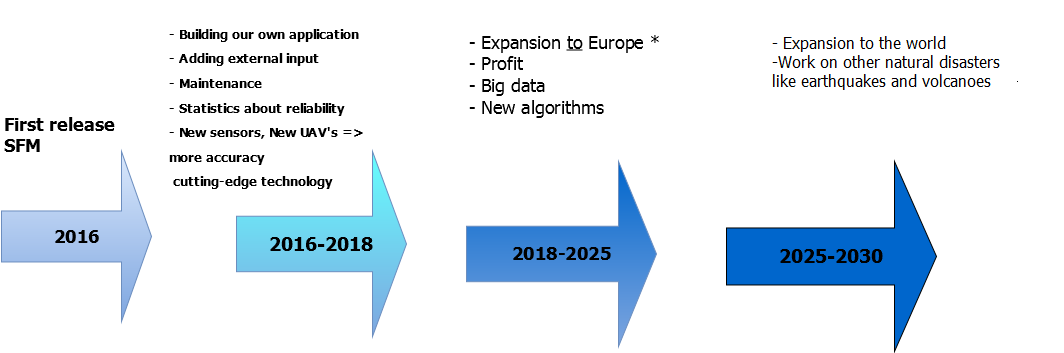
\includegraphics[scale=0.5]{images/Roadmap.png}
	\caption{Roadmap of \CompanyName{}}
	\label{fig:roadmap}
\end{figure}

*1 The statistics are made according to the goals in part 2.2. \\
*2 The expansion to Europe and the world is made by starting with countries which have high risk and history of floods (the team will get documentation, studies in order to choose countries which really need our product, countries where this market doesn't exist yet or at least isn't in expansion. This is a business strategy which should lead to more production and profit.\\

\section{System in the market}
All over the world floods are causing tremendous trouble to people. This makes that our system can be sold all over the world. First the system focuses on the Netherlands. When the system is working correctly other governments in the world must be informed about the system. First focusing on Europe and then other continents.

Third party application developers have the opportunity to build applications that enables guidance for emergency services and citizens. First, the focus is on finding one company that has experience with building such products. Then other software companies should get aware about the system. The more third party applications are build, the better system will reach its mission.

Safety regions are responsible when disasters are happening in the region. They consist of local governments, emergency services, the army and water boards. Safety regions and the organizations that are part of the safety regions should be informed about the system. When they know about the system they can inform the government and put pressure to buy this system.

When a flood is happening and things go wrong, inhabitants will ask governments what went wrong and state that they want to be better protected. They will pressure governments that they have the best flood warning system.

%\section{Business model}
%\ Insert a business model diagram
%\ Joris
%\section{Domain model}
%\ Internal how our system works?
%\ Joris
\section{Financial model}
The financial model will be a low product price. This in order to price the product low in the market. A service description for maintenance will be offered. Also updates will be sold to the customer.\\
%\Joris
\subsection{Software Architecture costs}
The software architecture team of \CompanyName consists of six members. Creating the architecture of the project is estimated to take ten weeks. All team members will spend 15 hours a week on the project. This totals $6*10*15=1050$ working hours. Each working hour costs \euro{}150,-. Total spend on the software architecture is \euro{}157.500.
%\Joris
\subsection{Development costs}
The costs of developing the system is approximated in table \ref{table:develop-costs}, shown below.

\begin{table}[H]
	\centering
	\begin{tabular}{lr}
	\toprule
	\textbf{Description} & \multicolumn{1}{l}{\textbf{Man hours}} \\ \hline
	Get values from various sensors & 160 \\ 
	Get weather forecasts & 160 \\ 
	Flood prediction algorithm & 3100 \\ 
	Warning messaging system  & 2000 \\ 
	Guidance information system & 1500 \\ 
	Redundancy and fail over systems & 1000 \\ 
	Testing \& debugging & 600 \\ 
	Release build & 250 \\
	Overhead & 1000 \\ 
	Total hours & 9770 \\
	\bottomrule
	\end{tabular}
	\caption{Approximation of development costs}
	\label{table:develop-costs}
\end{table}

%\Joris
Development of the system comprises the development of several different aspects. For each of these aspects, table \ref{table:develop-costs} shows an approximation of the hours needed for the development. Resulting in a total amount of $9770$ hours needed to create the system.\\
The development is done by \CompanyName self. Each member of the project team assigned to develop this system is paid $\euro{}50$ an hour. This results in a development cost of $50*9770=488.550$. As shown in the table below.

\todo{add the duration?}
%Members & 6 \\
%Duration & $\approx$41 weeks \\

% \pgfplotstableread%
% [%
% 	row sep=\\,
% 	col sep=&,
% 	format=inline
% ]%
% {\\%
% 	Description & Costs \\
% 	Hours & 9770 \\
% 	Cost per hour & \EUR{}50 \\
% 	Total cost & \EUR{}488.500 \\
% 	}\tdevcost

\begin{table}[H]
	\centering
	\begin{tabular}{lr}
	\toprule
	\textbf{Description} & \multicolumn{1}{l}{\textbf{Costs}} \\ \hline
	Hours & 9770 \\
	Cost per hour & \EUR{}50 \\
	Total cost & \EUR{}488.500 \\
	\bottomrule
	\end{tabular}
	\caption{Total costs of development}
	\label{table:total-dev-costs1}
\end{table}

\subsection{Hardware costs}
The hardware cost of the \gls{SFM} is separated in to dike sensors cost, water level sensor cost, maintenance cost, and server cost.

\subsubsection{Dike sensors}
Around 17.000 kilometers of dikes protect the Netherlands against flooding \cite{DMC}. 
The monitoring system consists of GeoBeads sensors with a claimed life time of 10 years, which are installed with conventional push-in techniques. 

The GeoBeads sensor costs about \EUR350 per unit. For every 3 meter of dike, one such sensor is needed. In the Netherlands, there are about 17.000 kilometers of dike. However, it is estimated that only about 2500km of the dikes have to be monitored by dike sensors (because the water board considers these dikes potentially unstable).

Each push-in costs about \EUR{}200 and three sensors can be installed per push-in\cite{TUDelftPHD}. %pp126

The following table gives an overview of the costs related to the dike sensors:

\begin{table}[H]
	% \pgfplotstabletypeset[
	% 	KeyValue
	% ]{%
	% 	Description & Value & UoM\\
	% 	Total length of all dikes to be monitored & $2.500$ & km \\
	% 	Number of GeoBeads per kilometer & 330 & \\
	% 	Sensor cost & 320 & \EUR{} \\
	% 	Installment cost per cross-section & 200 &\EUR{} \\
	% 	Sensors per cross-section & 3 & \\
	% 	Base installation cost factor like labor and wiring & 0.2 & \\
	% 	Life expectancy of GeoBeads & 10 & years \\
	% }


	\centering
	\begin{tabular}{lrl}
	\toprule
	\textbf{Description} & \multicolumn{1}{l}{\textbf{Value}} & \textbf{UoM} \\ \hline
	Total length of all dikes to be monitored & $2.500$ & km \\
	Number of GeoBeads per kilometer & 330 & \\
	Sensor cost & 320 & \EUR{} \\
	Installment cost per cross-section & 200 &\EUR{} \\
	Sensors per cross-section & 3 & \\
	Base installation cost factor like labor and wiring & 0.2 & \\
	Life expectancy of GeoBeads & 10 & years \\
	\bottomrule
	\end{tabular}
	\label{table:total-dev-costs2} 
	\caption{Total costs of development. UoM=Unit of measurement}
\end{table}

This makes the costs for the dike monitoring as follows: \\
Initial cost per km: $ 330 * 320  +  (330 / 3) * 200 = \EUR127.600 * 1.2 = \EUR153.120$\\
Total initial cost: $ 153.120 * 2.500 = \EUR 382.800.000$

\subsubsection{Water level sensors}

The estimated price of the water level sensors is around 200 euro and the assumed number of required water level sensor is about one for every kilometer. In the Netherlands, the total length of the waterways is about $6000$ kilometers\cite{cbs-waterways}.

The following table gives an overview of the costs related to the dike sensors:

\begin{table}[H]
	% \pgfplotstabletypeset[
	% 	KeyValue
	% ]{%
	% 	Description & Value & UoM\\
	% 	Total length of waterways to be monitored & $6.000$ & km \\
	% 	Number of water level sensors per kilometer & 1 & \\
	% 	Sensor cost & 100 & \EUR{} \\
	% 	Installment cost & 100 &\EUR{} \\
	% 	Base installation cost factor like labor and wiring & 0.2 & \\
	% }

	\centering
	\begin{tabular}{lrl}
	\toprule
	\textbf{Description} & \multicolumn{1}{l}{\textbf{Value}} & \textbf{UoM} \\ \hline
	Total length of waterways to be monitored & $6.000$ & km \\
	Number of water level sensors per kilometer & 1 & \\
	Sensor cost & 100 & \EUR{} \\
	Installment cost & 100 &\EUR{} \\
	Base installation cost factor like labor and wiring & 0.2 & \\
	\bottomrule
	\end{tabular}
	\label{table:total-dev-costs3} 
	\caption{Total costs of water level sensors. UoM=Unit of measurement}
\end{table}

This makes the costs for the dike monitoring as follows: \\
$ 6.000 * 200 = \EUR1.200.000 * 1.2 = \EUR1.440.000$\\

\subsubsection{Arduino}
Based on the number of dike sensors and water level sensors, one arduino is needed for every kilometer. In this way 1 water level sensor can connect to the arduino, combined with multiple GeoBeads sensors. This means 6000 arduinos are needed. These arduinos can be bought in large amounts to press the costs. This results in a price of \EUR45 per arduino. In total this is $6.000 * \EUR45 = 270.000$

\subsubsection{Maintenance}


\newcommand{\installationCosts}{412.500.000}

The yearly maintenance costs for the dike sensors is estimated to be around \EUR$4.500.000$ per year. If the depreciation of the GeoBead sensor is added, this becomes $4.500.000 + 33*825.000 = \EUR31.725.000$. 

\subsubsection{Servers}
The \gls{SFM} will use two kind of clusters, those are analytics cluster and database clusters. Analytics cluster consist of six rack, while database clusters consist of four racks. This specification is written on section \ref{sec:hardware-description}. Each analytic rack has five server and one switch, while database cluster has two servers, three storage machines, and one switch. This cluster also needs cables and other materials in order to operate. Thus, the Server cost ($SC$) is calculated as follows:

\begin{equation*}
SC = (AC + DC + OC) \times 3
\end{equation*}

where $AC$ is analytic cluster cost, $DC$ is database cluster cost, and $OC$ is other cost. The cost will be multiplied by three because there are three data centers of this system. The other cost is assumed will be \EUR 1.500 and this cost is around cabling and other electrical needs. Table \ref{table:server-cost} depicts analytic and database cluster cost calculation.

\begin{table}[H]
\centering
\caption{Server cost calculation}
\label{table:server-cost}
\begin{tabular}{lrrrr}
\hline
\textit{Detail}  & \multicolumn{1}{l}{\textit{Cost}} & \multicolumn{1}{l}{\textit{Quantity}} & \multicolumn{1}{l}{\textit{Subquantity}} & \multicolumn{1}{l}{\textit{Total}} \\ \hline
\multicolumn{5}{l}{\textbf{Analytic cluster}}                                                                                                                                \\ \hline
Server rack      & 700                               & 6                                     & 1                                        & 4.200                              \\
Servers          & 1.880                             & 6                                     & 5                                        & 56.400                             \\
Switches         & 1.273                             & 6                                     & 1                                        & 7.638                              \\ \hline
\multicolumn{4}{r}{\textbf{Total}}                                                                                                      & \textit{\textbf{68.238}}           \\ \hline
\multicolumn{5}{l}{\textbf{Database cluster}}                                                                                                                                \\ \hline
Server racks     & 700                               & 4                                     & 1                                        & 2.800                              \\
Servers          & 1.880                             & 4                                     & 2                                        & 15.040                             \\
Storage machines & 1.149                             & 4                                     & 3                                        & 13.788                             \\
Switches         & 1.273                             & 4                                     & 1                                        & 5.092                              \\ \hline
\multicolumn{4}{r}{\textbf{Total}}                                                                                                      & \textit{\textbf{36.720}}          
\end{tabular}
\end{table}

Therefore. the total cost for server will be:

\begin{equation*}
SC = (AC + DC + OC) \times 3
\end{equation*}

\begin{equation*}
SC = (68.238 + 36.720 + 1.500) \times 3 = \EUR 319.374
\end{equation*}

\subsubsection{UAVs costs}

The price of the Airborne A2xA4 is 31.273$\euro{}$ and the system will use fifty UAVs . Total cost = $\euro{}$1.563.650. The number of UAVs released depends on the size of the flooded area but the system has fifty UAVs available. \\
The maintenance costs of the UAV for all of them are rising to $\euro{}$500 per UAV per year so for the first ten years of the project : 500*50*10=$\euro{}$250.000. \\
Three maintainers will receive a training to learn how to pilot the UAVs: 3.217*3= 9.651$\euro{}$. \\
Total costs : $\euro{}$1.796.301 . \\

%http://www.uxvuniversity.com/uav-pilot-training-certificate/
\subsubsection{Total hardware costs}
The total hardware costs is shown in the table below.
\begin{table}[H]
	% \pgfplotstabletypeset[
	% 	Costs
	% ]{
	% 	Description & Cost\\
	% 	Installation costs & $\EUR{}$384.240.000\\
	% 	Maintenance costs per year & $\euro{}$31.725.000\\
	% 	Server costs & $\euro{}$319.374\\
	% 	Total cost & $\euro{}$416.284.374\\
	% }

	\centering
	\begin{tabular}{lr}
	\toprule
	\textbf{Description} & \multicolumn{1}{l}{\textbf{Costs}} \\ \hline
	Installation costs & $\EUR{}$384.510.000\\
	Maintenance costs per year & $\euro{}$31.725.000\\
	Server costs & $\euro{}$319.374\\
	UAVs & $\euro{}$1.796.301\\
	Total cost & $\euro{}$418.350.675 \\
	

	\bottomrule
	\end{tabular}
	\caption{Total hardware cost}
	\label{table:total-hardw-cost}
\end{table}

\subsection{Total costs}
The total costs for the system is calculated in the table below.\\

\begin{table}[H]
	% \pgfplotstabletypeset[%
	% 	Costs
	% ]{%
	% 	Description & Cost\\
	% 	Software Architecture costs & \EUR{}157.500\\
	% 	Development costs & $\euro{}$488.500\\
	% 	Hardware costs & $\euro{}$416.284.374\\
	% 	Total cost & $\euro{}$416.930.374\\
	% }

	\centering
	\begin{tabular}{lr}
	\toprule
	\textbf{Description} & \multicolumn{1}{l}{\textbf{Costs}} \\ \hline
	Software Architecture costs & \EUR{}157.500\\
	Development costs & $\euro{}$488.500\\
	Hardware costs & $\euro{}$418.350.675\\
	Total cost & $\euro{}$418.996.675\\
	
	
	\bottomrule
	\end{tabular}
	\caption{Total cost of the system}
	\label{table:totalcosts}
\end{table}
So the total costs of the system is $\euro{}$418.996.675\\
% Guntur: Doubled financial model sections?
% \section{Financial model}
% The financial model will be a low product price. This in order to price the product low in the market. A service description for maintenance will be offered. Also updates will be sold to the customer

\section{Competitors}
Siemens is a competitor that already has developed a flood-warning system in Belgium in 2006. When the system detects an imminent flood it sends a SMS to people that live near the rivers in order to warn them. The system is implemented in a small region, which consists of only 3 rivers. The total costs for this system were \euro{}230.000. Later on they continued engineering the system. The system uses sensors which measures: temperature, water pressure, and shifting. They participated with this system in the Urban Flood project from the EU. The strong point of this competitor is that they already have funding and also experience with building such a system. Siemens is the main competitor for \CompanyName{}. Their strength is that they already have a proven system in Belgium and have a lot of experience through participating in flood monitoring research projects. The opportunity for \CompanyName{} is to engineer a flexible system that can be used in the future for other kind of disasters. Further on by selling the product at a low selling price and profit on the maintenance work and upgrades the Netherlands will be interesting in using the product.

Further there are Universities that do research on flood warning systems. At the Malaysian Institute Information Technology they developed a product prototype of a system called Intelligent Flood Information System via SMS. Water level sensors are the only one they used. When there is a flood they send a warning SMS to people that are within the area. In the future this could become a competitor if they create a start-up or sell the idea to a company.  

%\Joris can you put references in?

%http://www.researchgate.net/publication/239761436_Intelligent_flood_information_system_via_SMS_(IFIS)

%http://datanews.knack.be/ict/nieuws/sms-waarschuwt-voor-overstromingen-br/article-normal-317597.html
%http://www.urbanflood.eu/Pages/Newsletter6.aspx
%https://en.wikipedia.org/wiki/Flood_warning (examples)
%https://www.campbellsci.com/flood-warning (sensors)
